% PUMA TPC: native macOS build, DLC dispersion, pi/K reco, GENFIT vs UKF
% Compile: pdflatex PUMA_DLC_slides.tex  (needs beamer; figures in ./figs/)
\documentclass[aspectratio=169,10pt]{beamer}
\usetheme{Madrid}\usecolortheme{whale}
\usepackage{graphicx,booktabs}
\setbeamertemplate{navigation symbols}{}
\title[PUMA DLC / \(\pi\)K / GENFIT-UKF]{PUMA TPC — DLC dispersion, \(\pi/K\) reconstruction, GENFIT vs UKF}
\subtitle{Native macOS build: ROOT 6.32 / FairRoot v19 / Geant4 11.2 / GenFit 2.2}
\date{}
\begin{document}
\frame{\titlepage}

\begin{frame}{What is working on the Mac}
\begin{itemize}
\item[\checkmark] Full stack builds natively: FairSoft (ROOT 6.32.08, Geant4 11.2), FairRoot v19, ATTPCROOT, GenFit 2.2
\item[\checkmark] \textbf{PUMA Geant4 simulation runs} (fixed a Geant4-11.2 production-cut abort)
\item[\checkmark] \textbf{DLC resistive charge dispersion} from the measured sheet resistance
\item[\checkmark] \textbf{\(\pi^+\pi^-\) and \(K^+K^+\) sims + reconstruction} (pattern recognition)
\item[\checkmark] \textbf{GENFIT vs UKF comparison}: both fitters run (fixed an Eigen version mismatch that had excluded the UKF); \(\pi\) and \(K\) momentum/angle/vertex/charge results
\item[\checkmark] \textbf{PID study}: dE/dx K vs \(\pi\) separation (Bethe-Bloch) + charge-sign, and the DLC effect
\end{itemize}
\end{frame}

\begin{frame}{DLC dispersion --- the physics}
\begin{columns}
\column{0.52\textwidth}
\[ \sigma_{\mathrm{DLC}}=\sqrt{2t/(R\,C)} \]
\begin{itemize}
\item \(R\) = DLC sheet resistance = \textbf{1.2--1.5 M\(\Omega/\Box\)} (measured)
\item \(C\) = areal capacitance DLC\(\leftrightarrow\)pads (\(\sim6\times10^{-13}\) F/mm\(^2\))
\item \(t\approx\) shaping time (0.5 \(\mu\)s)
\end{itemize}
\small Replaces the origin package's \emph{assumed} \(RC=100\) ns/mm\(^2\). At 4 T gas diffusion is suppressed, so this term dominates.
\column{0.46\textwidth}
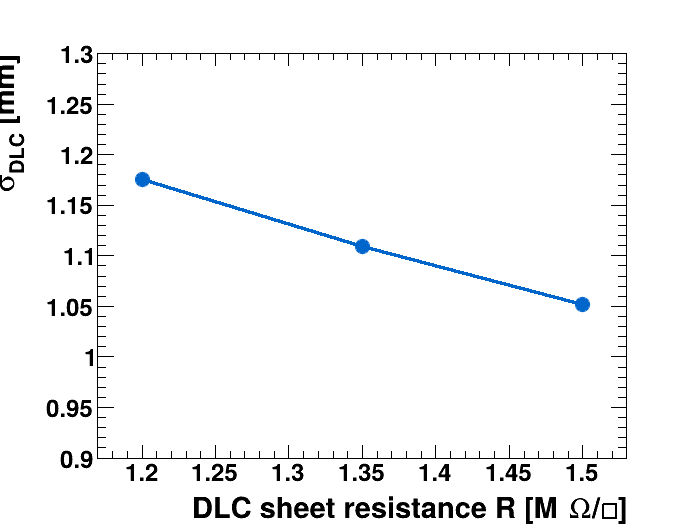
\includegraphics[width=\linewidth]{figs/sigma_vs_R.png}
\end{columns}
\end{frame}

\begin{frame}{DLC effect on digitization}
\begin{columns}
\column{0.5\textwidth}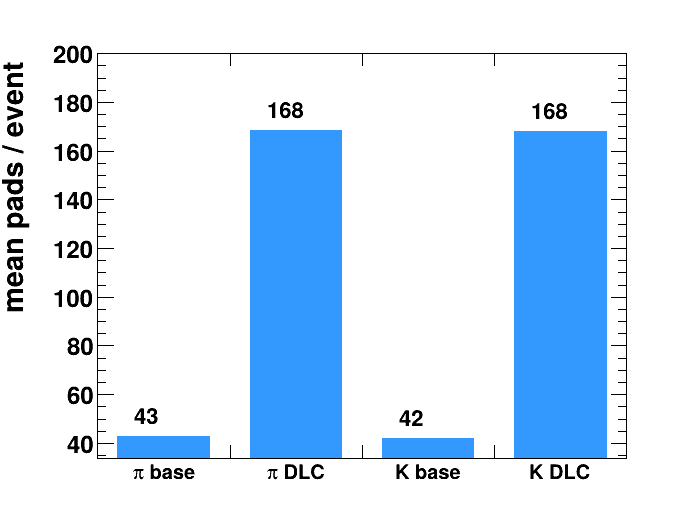
\includegraphics[width=\linewidth]{figs/pads_bar.png}
\column{0.5\textwidth}
\(\sigma_{\mathrm{DLC}}\approx1.0$--$1.2\) mm \(\Rightarrow\) charge over \(\sim\)1--2 pads \(\Rightarrow\) \textbf{\(\sim4\times\) pad multiplicity}.\\[.5em]
Previously the digitizer used base \texttt{AtPulse} with \emph{no} dispersion.\\[.5em]
Charge-conserving grid sub-sampling through the annular pad map \(\Rightarrow\) sub-pad centroiding.
\end{columns}
\end{frame}

\begin{frame}[fragile]{Pad pulses \& the PSA fit}
\centering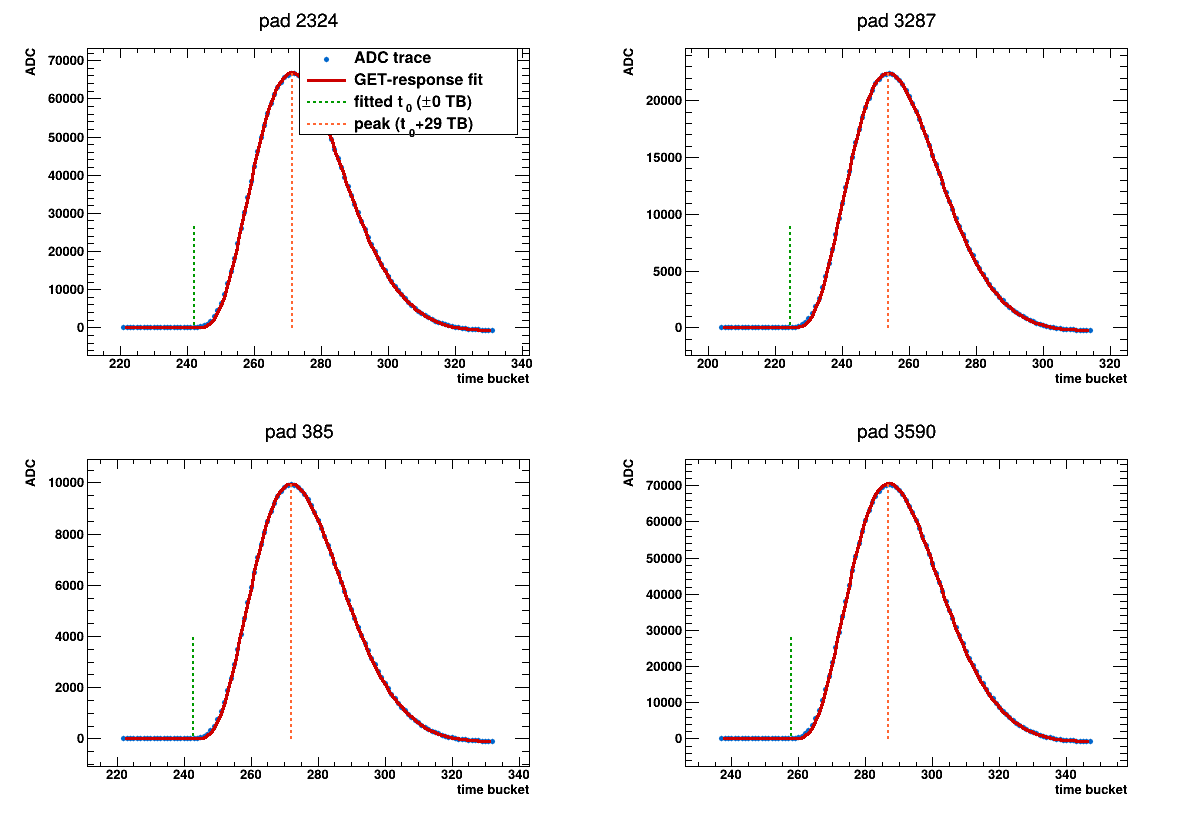
\includegraphics[height=.62\textheight]{figs/psa_fitshape.png}\\
{\small Pad traces (blue) with the \textbf{GET electronics-response fit} (red, \texttt{AtPSAMultiFit}: \(A\,e^{-3u}\sin u\,u^3\), \(u=(t-t_0)/\tau\), \(\tau=25\) TB) --- overlays the pulse shape \textbf{perfectly}. Fitted \textcolor{green!60!black}{impulse time \(t_0\)} = \textbf{unbiased} drift depth (\(z=\)vertex); \textcolor{orange}{response peak} lags \(t_0\) by the \(\sim\)8.6 mm shaping delay. \texttt{max}/\texttt{mfpeak}/\texttt{mfimpulse} all give \textbf{equivalent} \(\sim\)16--18\% momentum.}
\end{frame}

\begin{frame}{DLC in a real event (\(\pi^+\pi^-\))}
\centering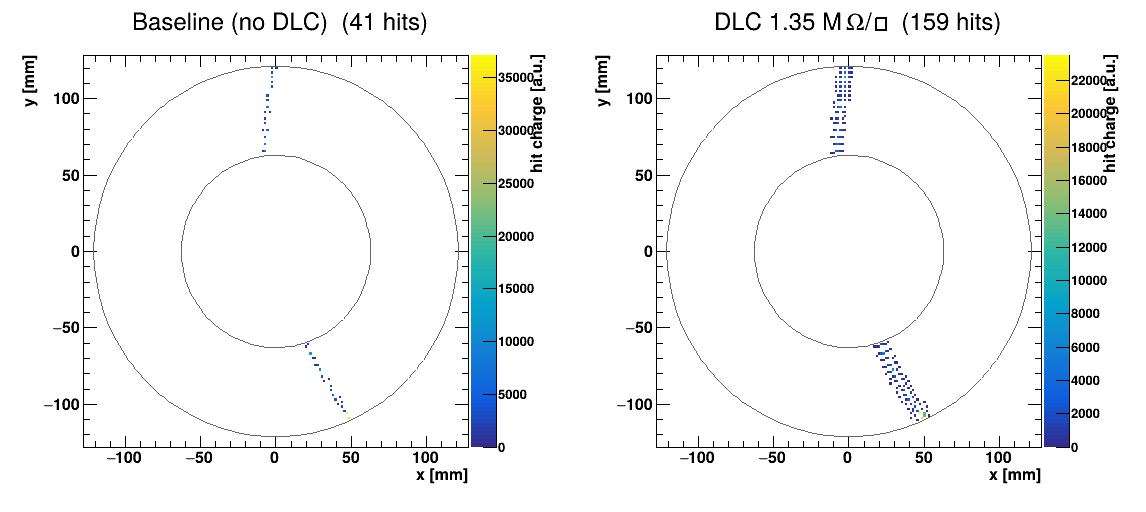
\includegraphics[height=.72\textheight]{figs/event_display.png}\\
{\small Same event, pads on a \textbf{charge (ADC) colour scale}: baseline (left, 41 pads) vs DLC (right, 159 pads). DLC spreads each cluster over \(\sim\)2 pads $\to$ lower per-pad amplitude but sub-pad centroiding.}
\end{frame}

\begin{frame}{Reconstructed tracks --- pad charge colour scale}
\centering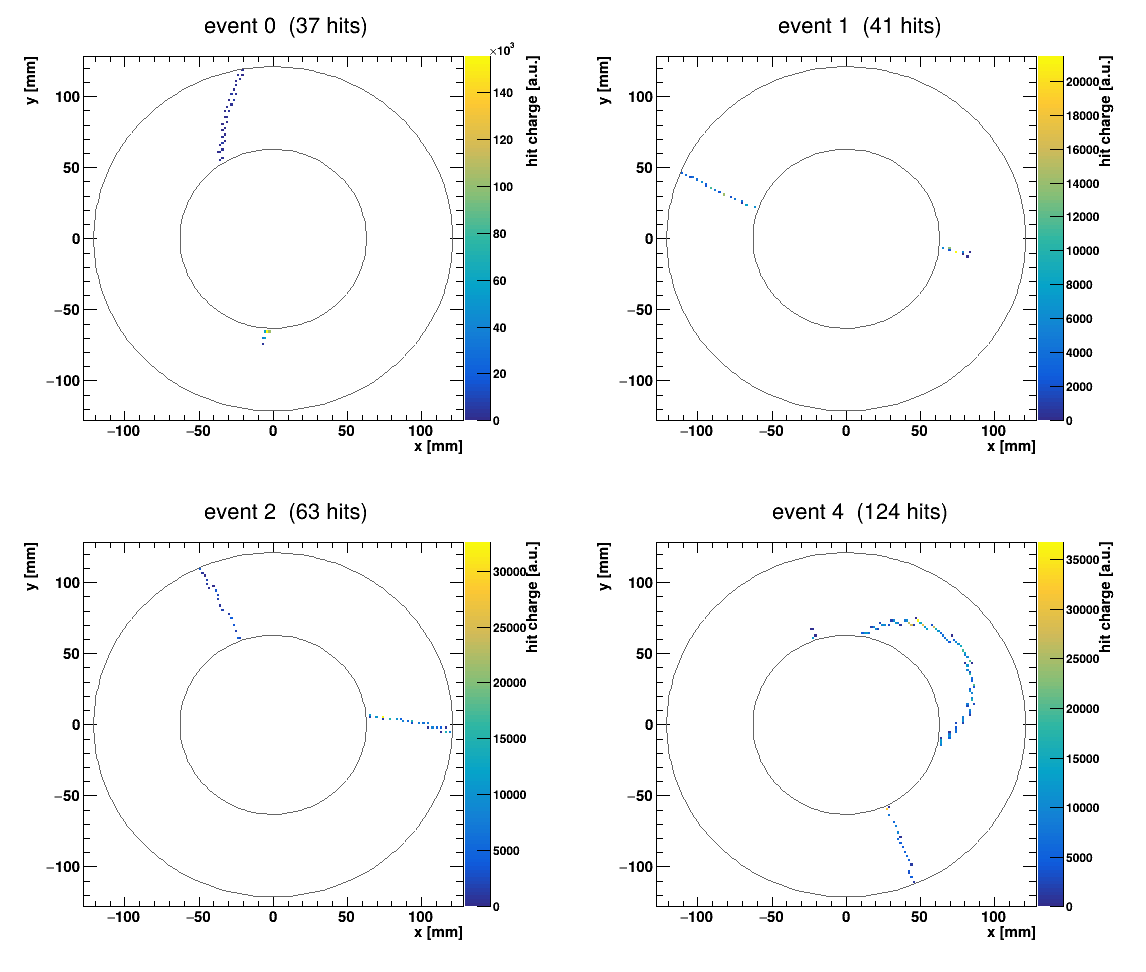
\includegraphics[height=.66\textheight]{figs/track_charge.png}\\
{\small Four events on the annular PUMA pad plane (R = 62.9--121.1 mm). Each hit/pad is drawn on a \textbf{charge (ADC) colour scale} (Z-axis palette = deposited charge/pad); tracks appear as the curved chains of fired pads, colour showing where ionization is heaviest. dE/dx = \(\Sigma Q_{\mathrm{pad}}\)/arc is built from exactly these values.}
\end{frame}

\begin{frame}{\(\pi\) and \(K\) simulations + reconstruction}
\begin{columns}
\column{0.55\textwidth}
\begin{table}\small\begin{tabular}{lccc}\toprule
Sample & pads/evt & tracks/evt & eff\\
 & base$\to$DLC & base$\to$DLC & \\\midrule
\(\pi^+\pi^-\) 0.4 GeV & 42.7$\to$168.3 & 2.08$\to$2.11 & 100\%\\
\(K^+K^+\) 0.777 GeV & 41.9$\to$168.1 & 1.52$\to$\textbf{1.25} & 100\%\\\bottomrule
\end{tabular}\end{table}
\small Same-charge kaons = mirror circles; DLC spreading slightly \textbf{merges} them in PRA (1.52$\to$1.25).
\column{0.45\textwidth}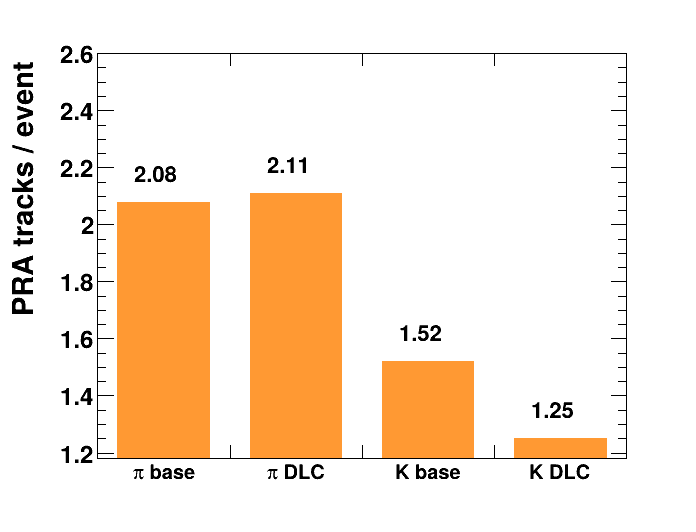
\includegraphics[width=\linewidth]{figs/tracks_bar.png}
\end{columns}
\end{frame}

\begin{frame}{UKF vs GENFIT --- pion resolution (150 evts)}
\centering
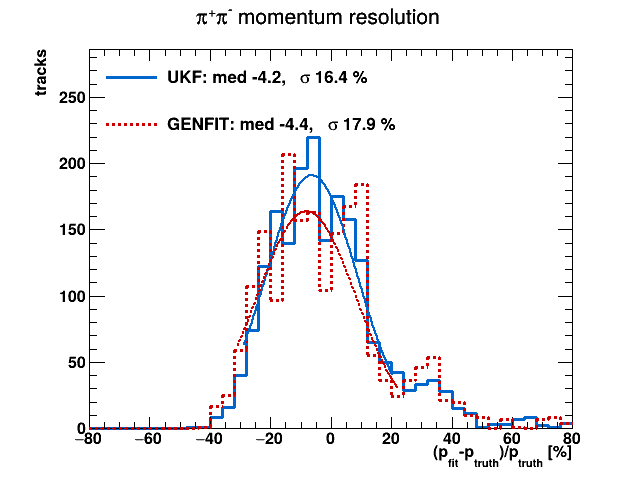
\includegraphics[height=.5\textheight]{figs/res_pi_dp.png}\hfill
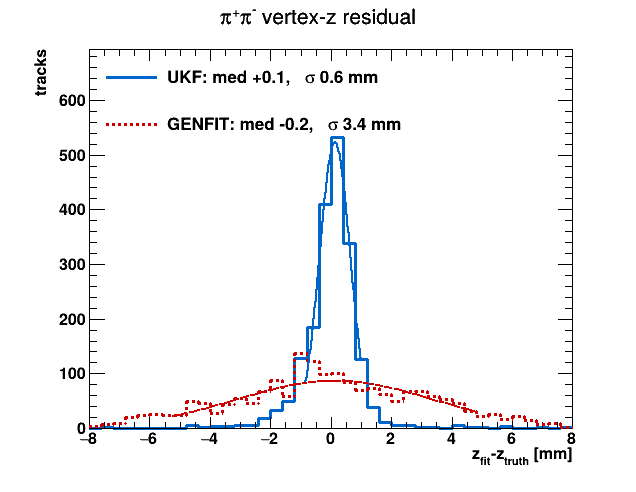
\includegraphics[height=.5\textheight]{figs/res_pi_vz.png}\\[.3em]
{\footnotesize\(\pi^+\pi^-\), \(|p|=374.9\) MeV/c, both fitters on \emph{identical} clusters.\quad
\begin{tabular}{lcccc}\toprule
 & p med/\(\sigma_{\mathrm{IQR}}\) & \(\theta\) \(\sigma\) & vtx \(\sigma_z\) & charge\\\midrule
UKF & -6.4/\textbf{18.0}\% & \textbf{1.9}\(^\circ\) & \textbf{0.63} mm & 99.2\%\\
GENFIT & -5.9/21.2\% & 2.6\(^\circ\) & 1.14 mm & 99.2\%\\\bottomrule
\end{tabular}}\\[.3em]
{\scriptsize Momentum \(\sim\)\textbf{18--21\%}, \(\theta\sim\textbf{2}^\circ\), charge \textbf{99\%}; \textbf{UKF vertex-z 2\(\times\) tighter}. \textbf{Per-ring centroiding} is the key reco choice; the PSA method (max / multi-fit) is equivalent. Robust median/\(\sigma_{\mathrm{IQR}}\).}
\end{frame}

\begin{frame}{UKF vs GENFIT --- kaons + per-ring clustering (150 evts)}
\centering
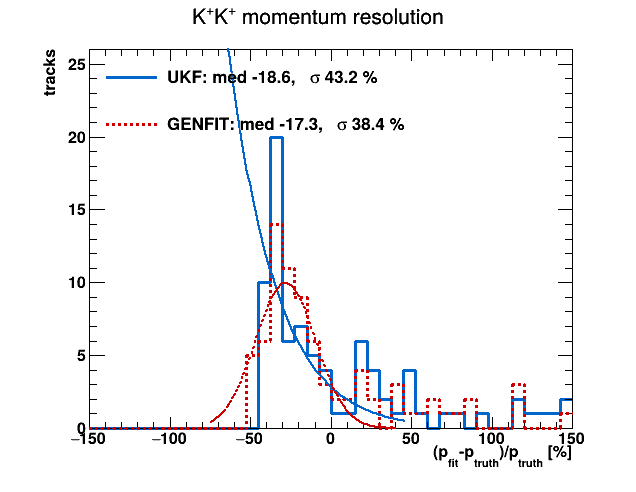
\includegraphics[height=.5\textheight]{figs/res_K_dp.png}\hfill
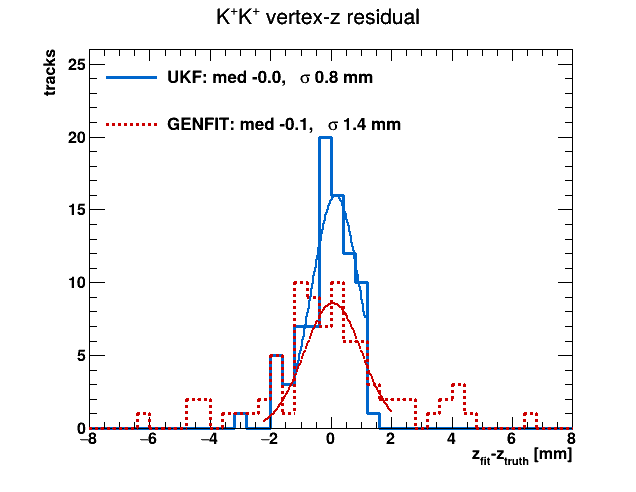
\includegraphics[height=.5\textheight]{figs/res_K_vz.png}\\[.3em]
{\footnotesize\(K^+K^+\), \(|p|=600\) MeV/c, per-ring resistive centroiding.\quad
\begin{tabular}{lcccc}\toprule
 & p med/\(\sigma_{\mathrm{IQR}}\) & \(\theta\) \(\sigma\) & vtx \(\sigma_z\) & charge\\\midrule
UKF & -18.6/43\% & 2.4\(^\circ\) & \textbf{0.78} mm & \textbf{100}\%\\
GENFIT & -17.3/\textbf{38}\% & 2.5\(^\circ\) & 1.42 mm & \textbf{100}\%\\\bottomrule
\end{tabular}}\\[.3em]
{\scriptsize \alert{Per-ring centroiding rescues the kaons:} the near-straight guard \emph{rejects} no-curvature tracks (keeps \textbf{45\%}, 78/174) $\to$ momentum \textbf{measurable} ($\sim$40\%) \& charge \textbf{100\%} (was $\sim$74\% no-ring). Quality-vs-efficiency: measure the well-curved half cleanly, drop the rest.}
\end{frame}

\begin{frame}{Particle ID --- dE/dx (K vs \(\pi\))}
\begin{columns}
\column{0.5\textwidth}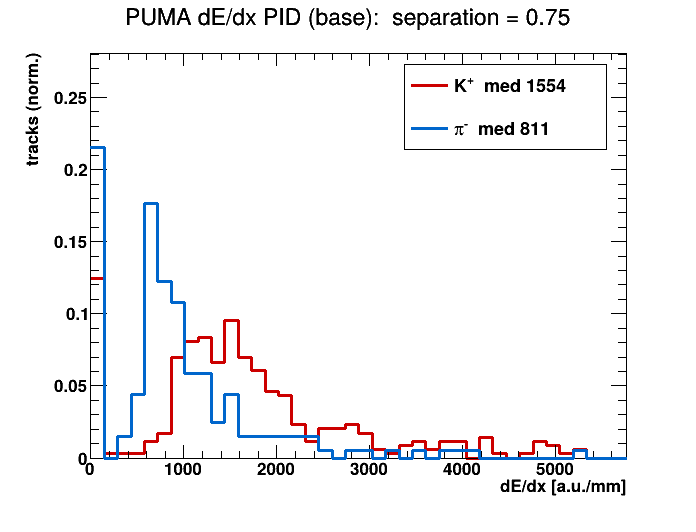
\includegraphics[width=\linewidth]{figs/pid_dedx_base.png}
\column{0.5\textwidth}
Full channel \(^3\)He+\(\bar p\to K^+K^+\pi^-\)+hex (both species/event, truth-labelled); dE/dx = \(\Sigma Q_\mathrm{hit}\)/arc:\\[.3em]
\begin{tabular}{lcccc}\toprule
 & K med & \(\pi\) med & K/\(\pi\) & sep\\\midrule
base & 1554 & 811 & 1.9\(\times\) & 0.75\(\sigma\)\\
DLC & 327 & 172 & 1.9\(\times\) & 0.72\(\sigma\)\\\bottomrule
\end{tabular}\\[.3em]
{\small K deposits \(\sim1.9\times\) the \(\pi\) dE/dx (Bethe-Bloch), \(\sim0.75\sigma\) separation. \alert{DLC} rescales dE/dx but leaves separation unchanged. Charge-sign (prev.\ slide) completes the PID.}
\end{columns}
\end{frame}

\begin{frame}{PID map --- dE/dx vs B\(\rho\)}
\begin{columns}
\column{0.5\textwidth}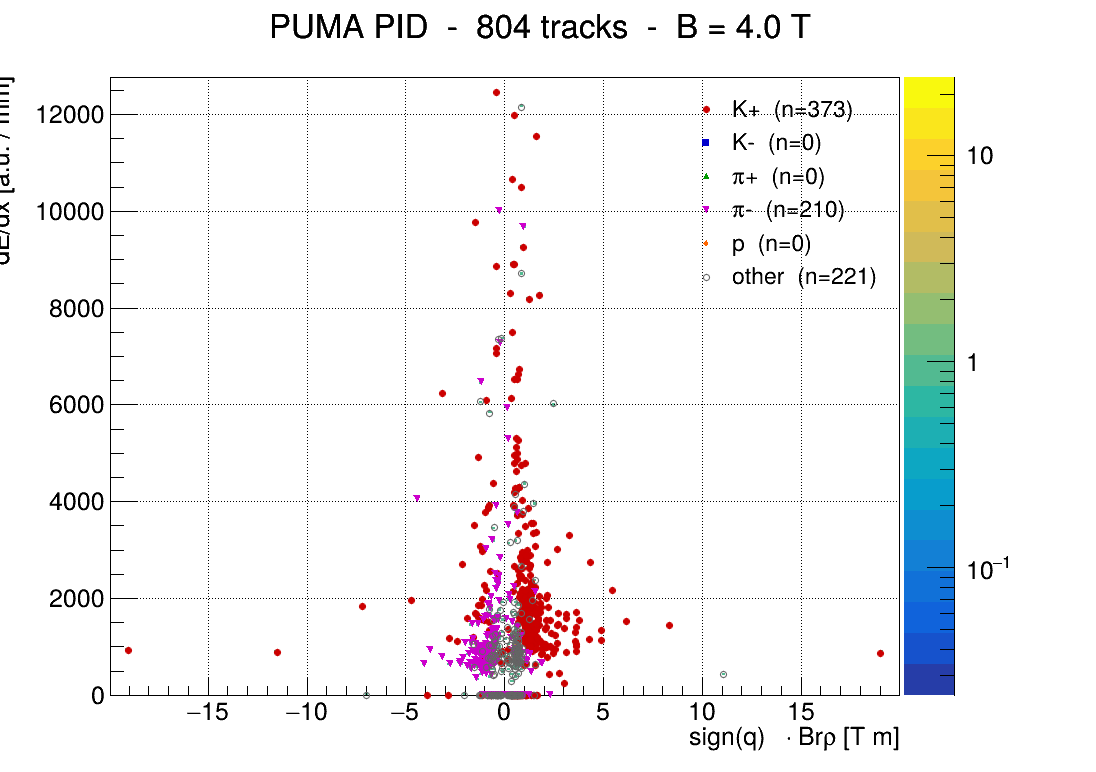
\includegraphics[width=\linewidth]{figs/pid_base.png}
\column{0.5\textwidth}
The classic 2D PID map: \textbf{dE/dx} vs \(\mathrm{sign}(q)\cdot B\rho\), with \(B\rho=B\,R/1000\) [T\,m] from the fitted circle radius \(R\) in 4 T.\\[.4em]
Two handles combine: \textbf{charge sign} splits the plane left/right (\(\pi^-\) vs K\(^+\)); \textbf{dE/dx} (vertical) adds the mass ordering (K\(^+\) \(\sim1.9\times\) higher).\\[.4em]
{\small Truth-labelled, full \(K^+K^+\pi^-\)+hex channel: \textcolor{red}{K\(^+\)} (\(n=373\)), \textcolor{blue}{\(\pi^-\)} (\(n=210\)). The plot a real analysis cuts on; K\(^+\)K\(^+\) merging populates the residual overlap.}
\end{columns}
\end{frame}

\begin{frame}[fragile]{How the fitter comparison was unblocked}
The UKF was \emph{never compiled} --- root cause was an \textbf{Eigen version mismatch}:
\begin{itemize}
\item brew installed \textbf{Eigen 5.0.1}; ATTPCROOT does \texttt{find\_package(Eigen3 3.3)}. Eigen 5.x is declared incompatible with a 3.3 request $\to$ \texttt{Eigen3::Eigen} target never created $\to$ the \texttt{if(TARGET Eigen3::Eigen)} block (AtFitterUKF, OpenKF) skipped $\to$ symbol absent from lib \& dictionary.
\item \textbf{Fix:} installed \textbf{Eigen 3.4.0}, prioritised over brew's. Rebuilt $\to$ UKF compiles $\to$ interpreted macro runs both fitters (as on Linux). Baked into \texttt{env.sh}.
\end{itemize}
\end{frame}

\begin{frame}[fragile]{Summary \& reproduce}
Native macOS PUMA chain sim\,$\to$\,digi(DLC)\,$\to$\,PSA\,$\to$\,PRA\,$\to$\,UKF/GENFIT works.\\
DLC 1.2--1.5 M\(\Omega/\Box\) $\to$ \(\sigma\approx1.0$--$1.2\) mm $\to$ $\sim4\times$ pads. Both fitters run, UKF\,$\approx$\,GENFIT.
\(\pi\): \(p\)-res $\sim$18--21\%, \(\theta\sim2^\circ\), charge 99\%. K: per-ring clustering $\to$ \(p\) measurable ($\sim$40\%), charge 100\% (45\% eff). Key reco knob = ring centroiding (PSA max/multi-fit equivalent).
\begin{block}{Reproduce (branch \texttt{puma-genfit-pion-mac})}
\scriptsize\begin{verbatim}
source build/config.sh
root -b -q 'PUMA_test8_sim.C(150,0.4)'     # pion sim (test10 -> kaon)
root -b -q 'run_digi_ukf_genfit_test8.C(150,8.,false,"max",\
   "pi",8,16,256,0.,true,true,false,20)'  # max PSA + ring clustering
root -b -q 'compare_ukf_genfit_test8.C("pi")'   # resolution numbers
root -b -q 'resolution_plots.C("pi")'           # dp/theta/vz figs
\end{verbatim}
\end{block}
\alert{Still to confirm:} \(C\) (DLC areal capacitance) --- the only free parameter in \(\sigma_{\mathrm{DLC}}\).
\end{frame}

\end{document}
